\chapter{システムの提案}
\label{chap:proposal}

本章では,音声利用についての背景を踏まえ,関連研究を概観し,新しい録音システム「Gyaon」を提案する.

\newpage

\section{設計指針}

「Gyaon」では
\begin{itemize}
\item 単純な録音操作
\item 音声管理の簡単さ
\item 他システムからの音声の利用のしやすさ
\end{itemize}
を優先した設計を行うことで録音の不便を解消し、音声の有効活用を促すシステムを目指している。

\section{利用例}
様々な利用シーンに対応するため、PC用Webアプリケーション\footnote{\textsf{https://gyaon.herokuapp.com/にて試験運用中}}および
Androidスマートフォン用アプリケーション
にてGyaonシステムを構築している。
それぞれのプラットフォームにおける利用例を述べる。

\subsection{PC版}

\paragraph{基本操作}
図\ref{button}の赤いボタンが録音ボタンであり、
長押しすることで録音を開始する。
ボタンを離すと録音が停止し、直ちに音声データがサーバへアップロードされる。
アップロードが完了したものは音声リスト(図\ref{list})に表示され、
マウスカーソルを重ねるだけで再生できる。

\begin{figure}[H]
\centering
\fbox{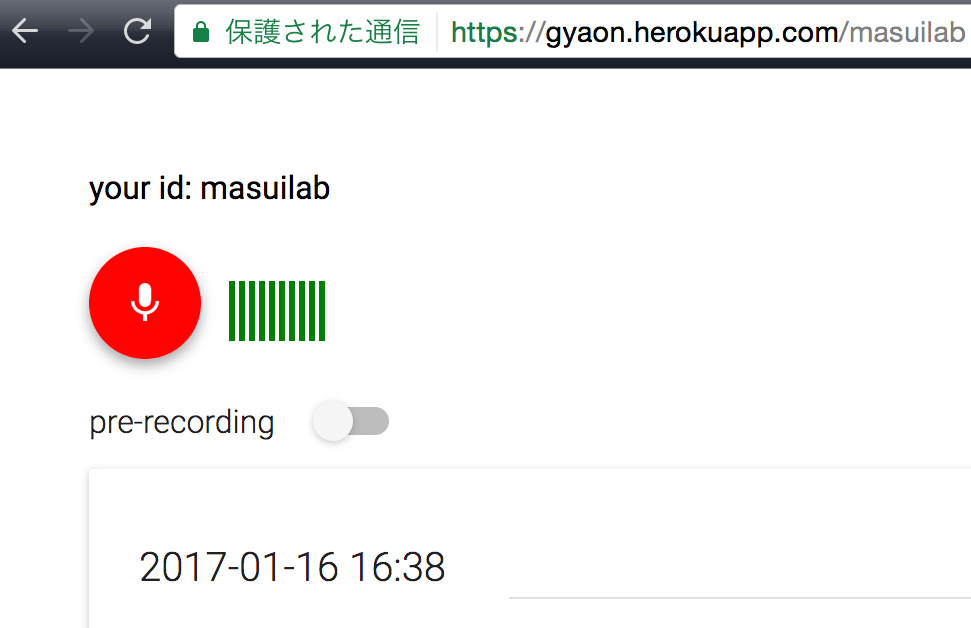
\includegraphics[width=9cm]{images/button.png}}
\caption{録音ボタン}
\label{button}
\end{figure}

\begin{figure}[H]
\centering
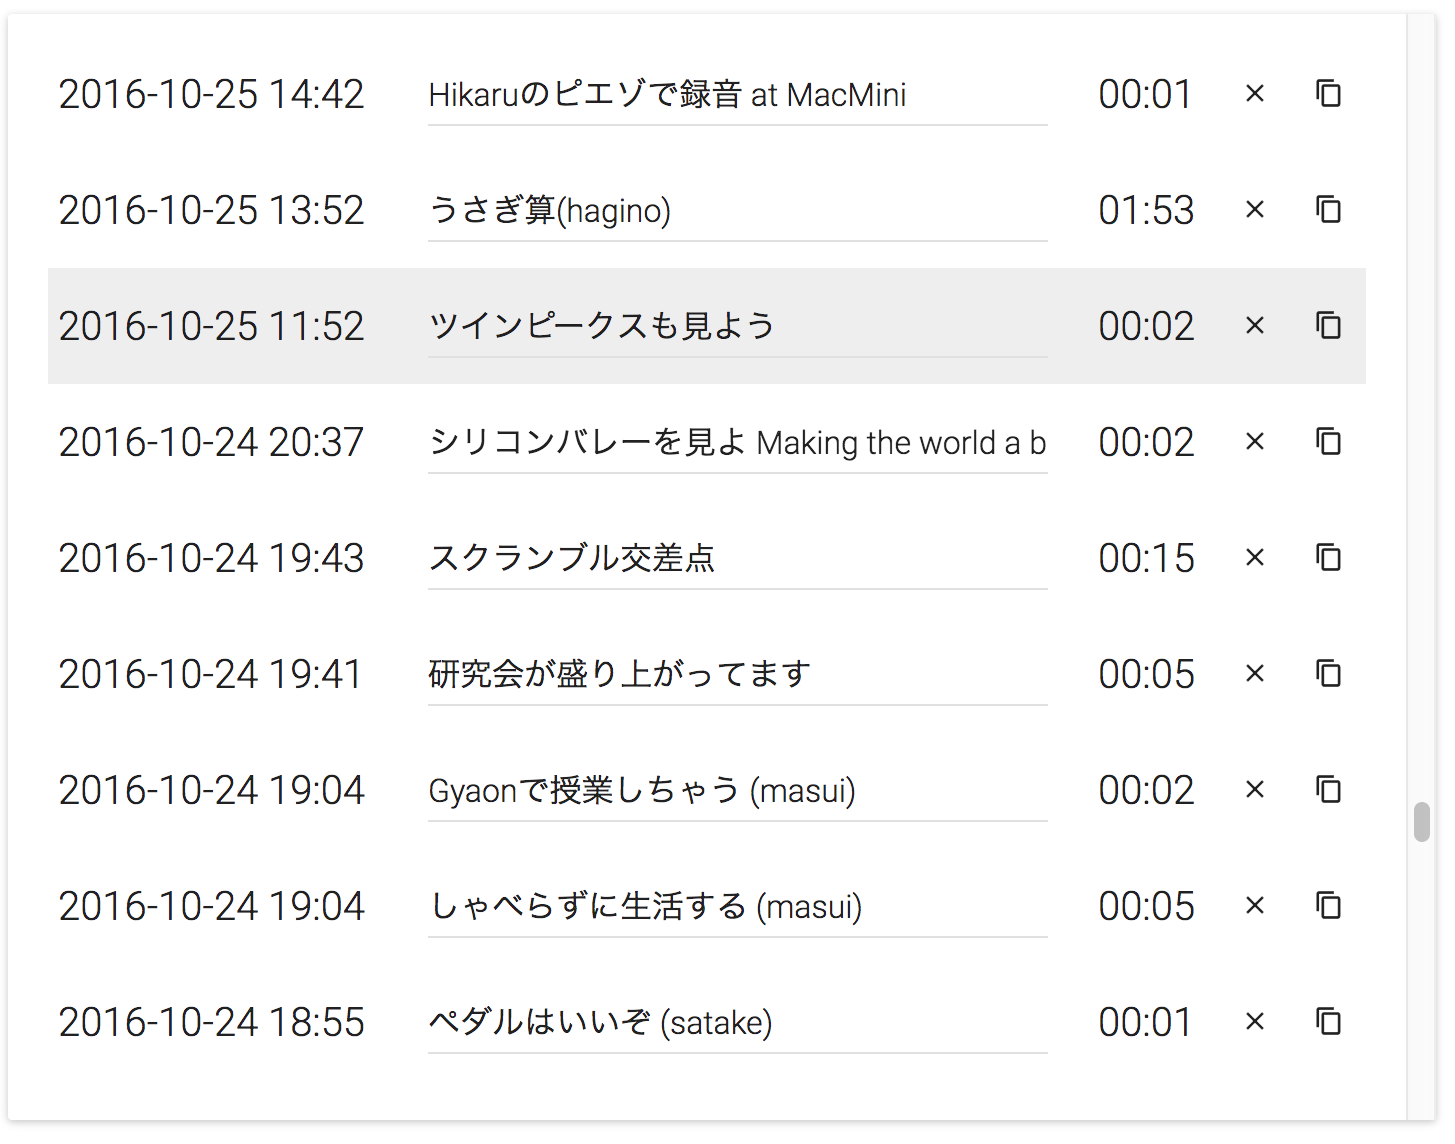
\includegraphics[width=9cm]{images/list.png}
\caption{音声リスト}
\label{list}
\end{figure}

\paragraph{コメントの追加}
音声リスト内にコメント入力欄があり、クリックすると入力モードに移行する。
音声の内容自由にメモを記録することができる。

\paragraph{音声URLの取得}
音声リストの右側のコピーボタンをクリックすることで、
PCのクリップボードに音声データのURLがコピーされる。
そのままアクセスすれば音声をダウンロードでき、ローカル環境のアプリケーションなどで利用できるほか、
URLを経由して他人に音声を渡すことも可能である。
またNota.inc\footnote{\textsf{http://www.notainc.com/ja/}}のWikiシステム
Scrapbox\footnote{\textsf{https://scrapbox.io/}}ではオーディオ記法を利用でき、
決められた書式で音声のURLを貼ると、Gyaonと同様にマウスカーソルによる音声の再生が可能となる。

\begin{figure}[H]
\centering
\fbox{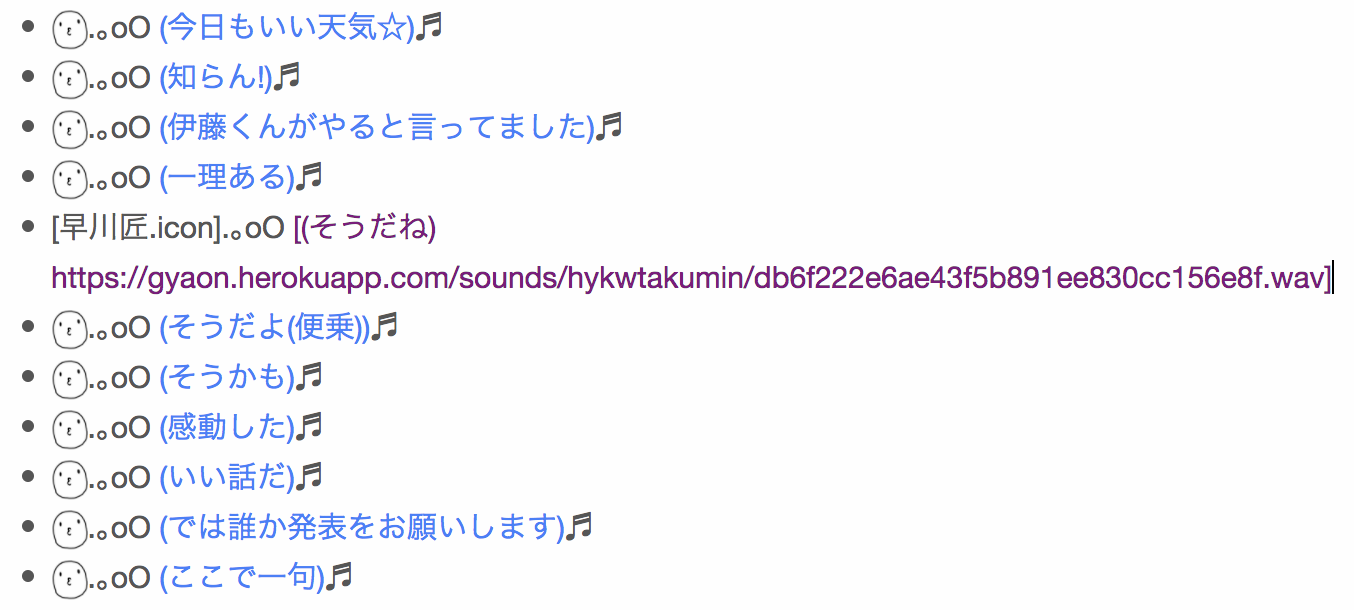
\includegraphics[width=9cm]{images/scrapbox.png}}
\caption{Scrapboxのオーディオ記法}
\label{scrapbox}
\end{figure}

\paragraph{プリレコーディング機能}
図\ref{button}のpre-recordingスイッチをONにするとアプリ起動中は常時録音し、
録音ボタンを押す10秒前から音声を記録できる。
撮りたい音を聞いてから録音ボタンを押しても間に合う
もし突然撮りたい音が聞こえてきた場合でも逃さず録音することが可能である。
%撮りたい音を逃さない
%今いいこと言った!を逃さない
%急に面白い音が聞こえてきても逃さない

\paragraph{地図機能}
音声データに紐付けられた位置情報をもとに、音声を地図上にマッピングして一覧できる
\footnote{\textsf{地図機能はhttps://gyaon.herokuapp.com/map/にて試験運用中}}。
ある音声がどの場所で撮影されたか分かることから、その場所の雰囲気や、
景色がいい/この店は美味しいといったその場所ならではの有用な情報を記録/共有できる。

\begin{figure}[H]
\centering
\fbox{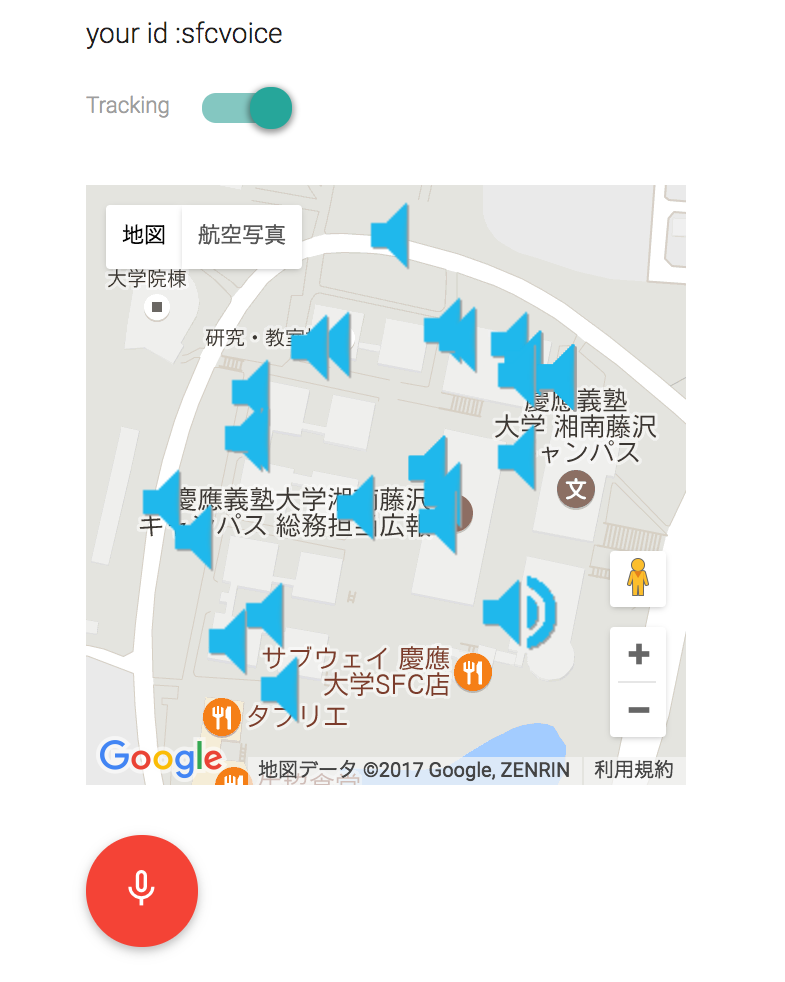
\includegraphics[width=9cm]{images/map.png}}
\caption{地図機能}
\label{map}
\end{figure}

\paragraph{IDの共有}
URL末尾はユーザIDとなっている
IDごとに音声を管理している
% ユーザIDを共有してコミュニケーションする
%  誰かが録音するとすぐに再生される

\paragraph{Gyaonキー}
アプリを起動しなくていい
%⌘+FNの画像

\paragraph{Gyaonペダル}
%  [satake 2016/10/24発表資料]
%  ハンズフリーで録音したいときに有用
%   楽器演奏
%   運転中
%   料理中?
%  Gyaon専用コンピュータとしてラズパイとかを繋げておけば小さいのでいろいろな所に置ける
%  ペダルはUSB接続の汎用品でいい
%  家とか研究室とかにばら撒いて使う
%   ペダルの画像

\subsection{Android版}
録音のみ可能
PC版と同じ録音インターフェースを持つ
ユーザIDを設定するとそこにアップする
同じIDを入れれば、スマホで撮った音をPCでも聞ける
図のように、画面に録音ボタンを常駐させておけるのでアプリを起動しなくても録音できる
撮り逃がさない
持ち運べるので、外で環境音を撮るのに向いてる
鳥のさえずり
川のせせらぎ
外で聞いた面白音声を共有する
電車遅延のアナウンスとか
街頭演説とか

%  アプリの画面のスクショ
%  常駐ボタンのスクショ
